\documentclass[10pt,pdf,hyperref=unicode,hyperref={bookmarks=false}]{beamer}

\usepackage{cmap}
\usepackage[T2A]{fontenc}
\usepackage[utf8]{inputenc}
\usepackage[english,russian]{babel}

\usetheme{Goettingen}
\title[Организация фестиваля Пива и Молока]{Управление проектом\\ <<Организация фестиваля Пива и Молока>>\\ с помощью Gantter.com}
%\author{Семенников Кирилл\thanks{\href{mailto:semennikovkirill@yandex.ru}{semennikovkirill@yandex.ru}} \and Чистяков Александр\thanks{\href{mailto:al.ol.chistyakov@gmail.com}{al.ol.chistyakov@gmail.com}}}
\author{Семенников Кирилл\and Чистяков Александр}
\institute{Санкт-Петербургский национальный исследовательский университет информационных технологий, механики и оптики}

\begin{document}
  \begin{frame}
    \maketitle
  \end{frame}
%  \begin{frame} \frametitle{План}
%    \tableofcontents
%  \end{frame}
  \section{Описание проекта}
    \begin{frame}{Цели проекта}
      \begin{itemize}
        \item Основная цель проекта:
          \begin{itemize}
            \item \emph{Организация и проведение фесиваля Пива и Молока 1~апреля~2014~года в городе Санкт-Петербург}
          \end{itemize}
        \item Глобальные цели проекта:
          \begin{itemize}
            \item{Оздоровление населения города Санкт-Петербурга.}
            \item{Формирование имиджа города Санкт-Петербурга как культурной столицы России.}
            \item{Эффективное перераспределение бюджетных средств.}
          \end{itemize}
      \end{itemize}
    \end{frame} 
    \begin{frame}{Устав проекта}
      Устав проекта включает следующие разделы:
      \begin{itemize}
        \item Общая информация
        \item Цели проекта
        \item Обоснование целесообразности проекта
        \item Основные этапы проекта
        \item Ресурсы проекта
        \item Риски проекта
        \item Ограничения
      \end{itemize}

      Последняя версия устава проекта доступна для загрузки:\\
      \href{https://github.com/chistyakov/pm/blob/master/charter.pdf?raw=true}{https://github.com/chistyakov/pm/blob/master/charter.pdf?raw=true}
    \end{frame}
  \section{Работа в системе Gantter.com}
    \begin{frame}[allowframebreaks]{Этапы и задачи}
  %\begin{frame}{Этапы и задачи}
%    \begin{figure}
%    \begin{figure}
      \begin{center}
        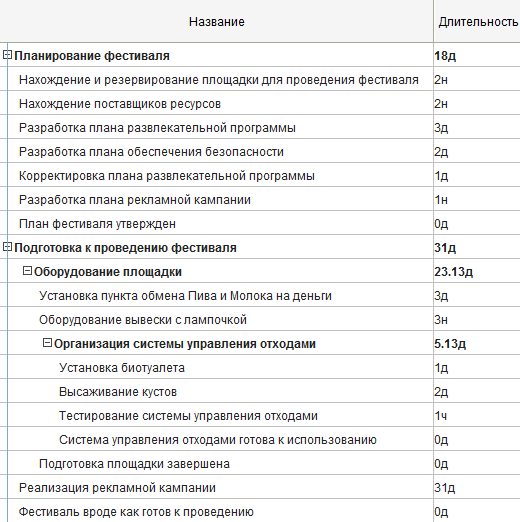
\includegraphics[keepaspectratio=true,width=\textwidth,height=0.8\textheight]{tasks1.png}\\
        \framebreak
        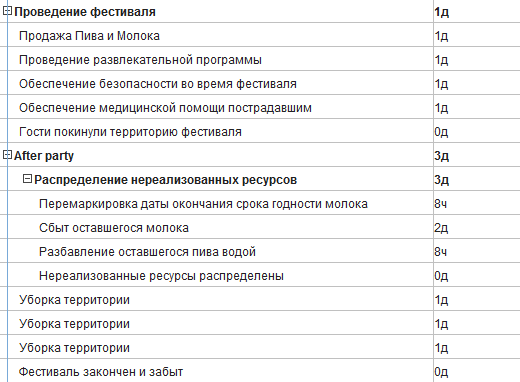
\includegraphics[keepaspectratio=true,width=\textwidth,height=0.8\textheight]{tasks2.png}
      \end{center}
%    \end{figure}
%      \framebreak
%    \begin{figure}
%      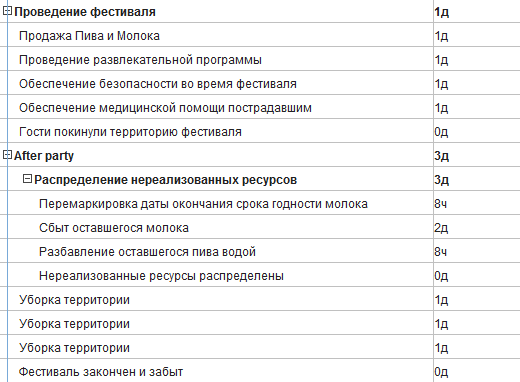
\includegraphics[keepaspectratio=true,width=\textwidth,height=\textheight]{tasks2.png}
%    \end{figure}
%    \end{figure}
%\newpage
%    \begin{figure}
      %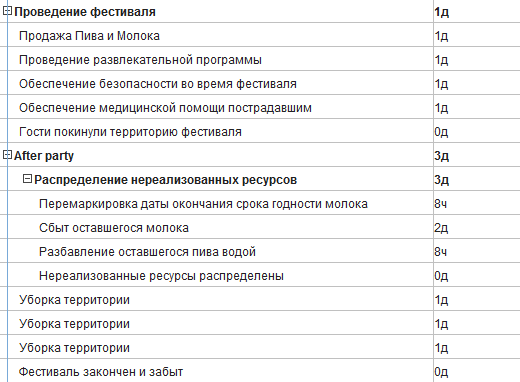
\includegraphics[keepaspectratio=false,width=\textwidth,height=\textheight]{tasks2.png}
%    \end{figure}
    \end{frame}
    \begin{frame}{Ресурсы}
    \end{frame}
    \begin{frame}{Риски}
    \end{frame}
    \begin{frame}{Базовый план}
    \end{frame}
  \section*{}
  \begin{frame}{Спасибо за внимание!}
    \begin{figure}
      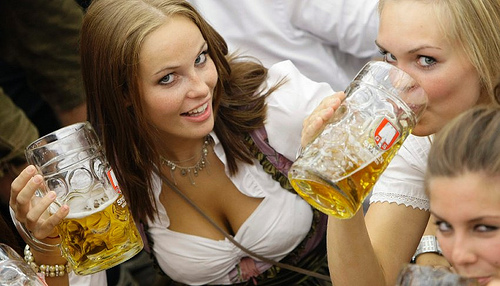
\includegraphics[width=\textwidth]{beers1.jpg}
    \end{figure}
  \end{frame}
\end{document}
